\section{Datos}

\subsection{Descripción de las fuentes de datos a utilizar}

El juego de datos ha sido obtenido de kaggle \cite{potholedataset} y se compone de un total de 1900 imágenes, tomadas desde el interior de un coche, con un tamaño igual a 3680x2760 píxeles (formato 4:3), y de un conjunto de ficheros de texto con el etiquetado de las mismas. Las imágenes se dividen en dos subconjuntos: uno de 1297 imágenes para el entrenamiento y otro de 603 imágenes para la evaluación del modelo. Por cada uno de los subconjuntos de imágenes existe un fichero de texto con el etiquetado de las mismas. Cada una de las líneas del los ficheros de texto contiene las etiquetas de una imagen. La estructura de cada línea es la siguiente:

\begin{lstlisting}[frame=single,basicstyle=\ttfamily\footnotesize]
<IMG_PATH> <NUMBER_OF_LABELS>( <X0> <Y0> <WIDTH> <HEIGHT>)+
\end{lstlisting}

Para facilitar el posterior tratamiento, se ha realizado una transformación del formato de los ficheros de etiquetas al siguiente formato:

\begin{lstlisting}[frame=single,basicstyle=\ttfamily\footnotesize]
<IMG_PATH>( <X0>,<Y0>,<WIDTH>,<HEIGHT>,<CLASS>)+
\end{lstlisting}

\subsection{Estudio de los datos}

En una fase inicial se ha realizado un análisis del tamaño de los socavones con respecto al tamaño de la imagen. Esto es un aspecto importante a tener en cuenta de cara a determinar el algoritmo a utilizar para la detección de objetos. Los algoritmos de detección de objetos, en general se comportan peor cuanto más pequeños son los objetos a detectar.

Como se observa en la figura \ref{fig:potholesizes}, la mayoría de los socavones tienen una anchura inferior a 200 píxeles y una altura inferior a 50 píxeles. Este factor será tenido en cuenta en el preprocesamiento de las imágenes.

\begin{figure}[H]
	\centering
	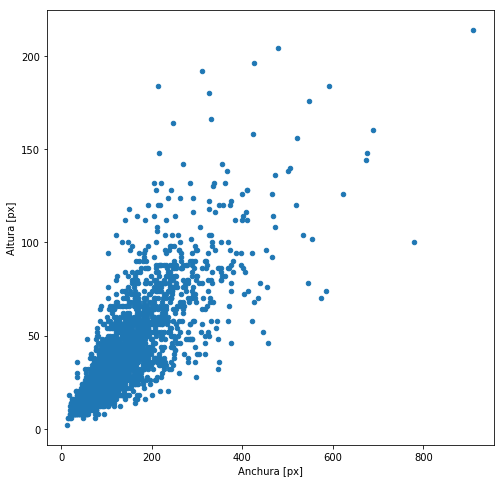
\includegraphics[width=0.8\linewidth]{images/pothole_sizes_scatter_plot.png}
	\caption{Tamaños de los socavones en píxeles}
	\label{fig:potholesizes}
\end{figure}

También se ha realizado un estudio de la localización de los socavones en las imágenes. Tal y como se ve en la figura \ref{fig:potholeslocations}, los baches están localizados principalmente en el centro de la imagen. La parte inferior se corresponde con el salpicadero del coche y la parte superior se corresponde con paisaje.

\begin{figure}[H]
	\centering
	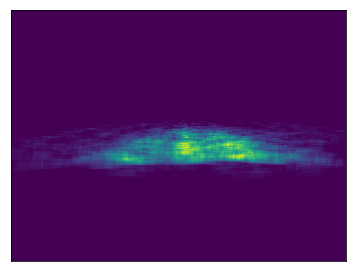
\includegraphics[width=0.8\linewidth]{images/pothole_locations_heatmap.png}
	\caption{Localizaciones de los socavones en las imágenes}
	\label{fig:potholeslocations}
\end{figure}

\subsection{Limpieza y normalización de los datos}

\textbf{!!! TODO}
\begin{itemize}
	\item explicar diferencia de tamaño entre redimensión directa vs crop + redimension
	\item explicar la normalización que se hace /255
	\item explicar el filtrado que se hace
\end{itemize}